% Options for packages loaded elsewhere
\PassOptionsToPackage{unicode}{hyperref}
\PassOptionsToPackage{hyphens}{url}
\PassOptionsToPackage{dvipsnames,svgnames,x11names}{xcolor}
%
\documentclass[
  ignorenonframetext,
]{beamer}
\usepackage{pgfpages}
\setbeamertemplate{caption}[numbered]
\setbeamertemplate{caption label separator}{: }
\setbeamercolor{caption name}{fg=normal text.fg}
\beamertemplatenavigationsymbolsempty
% Prevent slide breaks in the middle of a paragraph
\widowpenalties 1 10000
\raggedbottom

\usepackage{amsmath,amssymb}
\usepackage{iftex}
\ifPDFTeX
  \usepackage[T1]{fontenc}
  \usepackage[utf8]{inputenc}
  \usepackage{textcomp} % provide euro and other symbols
\else % if luatex or xetex
  \usepackage{unicode-math}
  \defaultfontfeatures{Scale=MatchLowercase}
  \defaultfontfeatures[\rmfamily]{Ligatures=TeX,Scale=1}
\fi
\usepackage{lmodern}
\usetheme[]{AnnArbor}
\usecolortheme{dolphin}
\usefonttheme{structurebold}
\ifPDFTeX\else  
    % xetex/luatex font selection
\fi
% Use upquote if available, for straight quotes in verbatim environments
\IfFileExists{upquote.sty}{\usepackage{upquote}}{}
\IfFileExists{microtype.sty}{% use microtype if available
  \usepackage[]{microtype}
  \UseMicrotypeSet[protrusion]{basicmath} % disable protrusion for tt fonts
}{}
\makeatletter
\@ifundefined{KOMAClassName}{% if non-KOMA class
  \IfFileExists{parskip.sty}{%
    \usepackage{parskip}
  }{% else
    \setlength{\parindent}{0pt}
    \setlength{\parskip}{6pt plus 2pt minus 1pt}}
}{% if KOMA class
  \KOMAoptions{parskip=half}}
\makeatother
\usepackage{xcolor}
\newif\ifbibliography
\setlength{\emergencystretch}{3em} % prevent overfull lines
\setcounter{secnumdepth}{-\maxdimen} % remove section numbering


\providecommand{\tightlist}{%
  \setlength{\itemsep}{0pt}\setlength{\parskip}{0pt}}\usepackage{longtable,booktabs,array}
\usepackage{calc} % for calculating minipage widths
\usepackage{caption}
% Make caption package work with longtable
\makeatletter
\def\fnum@table{\tablename~\thetable}
\makeatother
\usepackage{graphicx}
\makeatletter
\def\maxwidth{\ifdim\Gin@nat@width>\linewidth\linewidth\else\Gin@nat@width\fi}
\def\maxheight{\ifdim\Gin@nat@height>\textheight\textheight\else\Gin@nat@height\fi}
\makeatother
% Scale images if necessary, so that they will not overflow the page
% margins by default, and it is still possible to overwrite the defaults
% using explicit options in \includegraphics[width, height, ...]{}
\setkeys{Gin}{width=\maxwidth,height=\maxheight,keepaspectratio}
% Set default figure placement to htbp
\makeatletter
\def\fps@figure{htbp}
\makeatother
% definitions for citeproc citations
\NewDocumentCommand\citeproctext{}{}
\NewDocumentCommand\citeproc{mm}{%
  \begingroup\def\citeproctext{#2}\cite{#1}\endgroup}
\makeatletter
 % allow citations to break across lines
 \let\@cite@ofmt\@firstofone
 % avoid brackets around text for \cite:
 \def\@biblabel#1{}
 \def\@cite#1#2{{#1\if@tempswa , #2\fi}}
\makeatother
\newlength{\cslhangindent}
\setlength{\cslhangindent}{1.5em}
\newlength{\csllabelwidth}
\setlength{\csllabelwidth}{3em}
\newenvironment{CSLReferences}[2] % #1 hanging-indent, #2 entry-spacing
 {\begin{list}{}{%
  \setlength{\itemindent}{0pt}
  \setlength{\leftmargin}{0pt}
  \setlength{\parsep}{0pt}
  % turn on hanging indent if param 1 is 1
  \ifodd #1
   \setlength{\leftmargin}{\cslhangindent}
   \setlength{\itemindent}{-1\cslhangindent}
  \fi
  % set entry spacing
  \setlength{\itemsep}{#2\baselineskip}}}
 {\end{list}}
\usepackage{calc}
\newcommand{\CSLBlock}[1]{\hfill\break\parbox[t]{\linewidth}{\strut\ignorespaces#1\strut}}
\newcommand{\CSLLeftMargin}[1]{\parbox[t]{\csllabelwidth}{\strut#1\strut}}
\newcommand{\CSLRightInline}[1]{\parbox[t]{\linewidth - \csllabelwidth}{\strut#1\strut}}
\newcommand{\CSLIndent}[1]{\hspace{\cslhangindent}#1}

\usepackage{booktabs}
\usepackage{longtable}
\usepackage{array}
\usepackage{multirow}
\usepackage{wrapfig}
\usepackage{float}
\usepackage{colortbl}
\usepackage{pdflscape}
\usepackage{tabu}
\usepackage{threeparttable}
\usepackage{threeparttablex}
\usepackage[normalem]{ulem}
\usepackage{makecell}
\usepackage{xcolor}

% logo
\titlegraphic{
\includegraphics[width=4cm]{000_logos/logo-blue-vertical}}
\logo{\ifnum\thepage>1
\includegraphics[width=0.5cm]{000_logos/logo-blue-vertical}\fi}

% UMNG: Manual de image institucional

% Colors

% Umng
\definecolor{yellow}{HTML}{fdc600}
\definecolor{red}{HTML}{ee2a24}

% Estudios a Distancia
\definecolor{blue1}{HTML}{12245b}
\definecolor{blue2}{HTML}{767ca6}
\definecolor{blue3}{HTML}{cad2ec}

% Modify items
\setbeamercolor{palette primary}{bg=blue3}
\setbeamercolor{palette tertiary}{bg=blue1}
\setbeamercolor{frametitle}{bg=yellow}

% Hyperlinks
\hypersetup{
  linkcolor=red,
  citecolor=red
}

\makeatletter
\@ifpackageloaded{caption}{}{\usepackage{caption}}
\AtBeginDocument{%
\ifdefined\contentsname
  \renewcommand*\contentsname{Table of contents}
\else
  \newcommand\contentsname{Table of contents}
\fi
\ifdefined\listfigurename
  \renewcommand*\listfigurename{List of Figures}
\else
  \newcommand\listfigurename{List of Figures}
\fi
\ifdefined\listtablename
  \renewcommand*\listtablename{List of Tables}
\else
  \newcommand\listtablename{List of Tables}
\fi
\ifdefined\figurename
  \renewcommand*\figurename{Figure}
\else
  \newcommand\figurename{Figure}
\fi
\ifdefined\tablename
  \renewcommand*\tablename{Table}
\else
  \newcommand\tablename{Table}
\fi
}
\@ifpackageloaded{float}{}{\usepackage{float}}
\floatstyle{ruled}
\@ifundefined{c@chapter}{\newfloat{codelisting}{h}{lop}}{\newfloat{codelisting}{h}{lop}[chapter]}
\floatname{codelisting}{Listing}
\newcommand*\listoflistings{\listof{codelisting}{List of Listings}}
\makeatother
\makeatletter
\makeatother
\makeatletter
\@ifpackageloaded{caption}{}{\usepackage{caption}}
\@ifpackageloaded{subcaption}{}{\usepackage{subcaption}}
\makeatother

\ifLuaTeX
\usepackage[bidi=basic]{babel}
\else
\usepackage[bidi=default]{babel}
\fi
\babelprovide[main,import]{english}
% get rid of language-specific shorthands (see #6817):
\let\LanguageShortHands\languageshorthands
\def\languageshorthands#1{}
\ifLuaTeX
  \usepackage{selnolig}  % disable illegal ligatures
\fi
\usepackage{bookmark}

\IfFileExists{xurl.sty}{\usepackage{xurl}}{} % add URL line breaks if available
\urlstyle{same} % disable monospaced font for URLs
\hypersetup{
  pdftitle={Best Practices in Negotiations},
  pdfauthor={Luis Francisco Gómez López},
  pdflang={en},
  colorlinks=true,
  linkcolor={Maroon},
  filecolor={Maroon},
  citecolor={Blue},
  urlcolor={Blue},
  pdfcreator={LaTeX via pandoc}}


\title{Best Practices in Negotiations}
\author{Luis Francisco Gómez López}
\date{2024-07-27}
\institute{FAEDIS}

\begin{document}
\frame{\titlepage}

\renewcommand*\contentsname{Table of contents}
\begin{frame}[allowframebreaks]
  \frametitle{Table of contents}
  \tableofcontents[hideallsubsections]
\end{frame}

\section{Please Read Me}\label{please-read-me}

\begin{frame}{}
\phantomsection\label{section}
\begin{itemize}
\item
  Check the message \textbf{Welcome greeting} published in the News
  Bulletin Board.
\item
  Dear student please edit your profile uploading a photo where your
  face is clearly visible.
\item
  The purpose of the virtual meetings is to answer questions and not to
  make a summary of the study material.
\item
  This presentation is based on
  (\citeproc{ref-lewicki_negociacion_2024}{Lewicki, Barry, and Saunders
  2024, chap. 20})
\end{itemize}
\end{frame}

\section{Purpose}\label{purpose}

\begin{frame}{}
\phantomsection\label{section-1}
Explore best practices in negotiation and conflict management to achieve
successful negotiation.
\end{frame}

\section{Final Exam Three Party Coalition Exercise
Modified}\label{final-exam-three-party-coalition-exercise-modified}

\begin{frame}{}
\phantomsection\label{section-2}
\begin{itemize}
\item
  Why the Final Exam is a simulations and with the participation of the
  entire course?

  \begin{itemize}
  \item
    The negotiation of conflicts is generated between individuals or
    groups and one way of learning is precisely by negotiating with
    other people.
  \item
    It is not effective to learn individually and only theoretically.
  \item
    It is as if a person learned theoretically to play football and
    without ever playing in a team. Most likely, that person will not
    perform well in a real match.
  \end{itemize}
\item
  Before taking part, students should review the general and specific
  instructions of the Final Exam that can be checked at:

  \begin{itemize}
  \tightlist
  \item
    Tercer corte 40\% \textgreater{} Learning Activities \textgreater{}
    Final Exam Three Party Coalition Exercise Modified
  \end{itemize}
\end{itemize}
\end{frame}

\begin{frame}{}
\phantomsection\label{section-3}
\begin{itemize}
\item
  Also check out in the \textbf{Links of interest} the
  videos\footnote<.->{The videos are in english and are recordings of
    the Three-Party Coalition Exercise simulation}

  \begin{itemize}
  \tightlist
  \item
    \emph{Three-Party Coalition Exercise}
    (\citeproc{ref-program_on_negotiation_negotiation_2014}{Program on
    Negotiation 2014a}) and
    (\citeproc{ref-program_on_negotiation_negotiation_2014-1}{Program on
    Negotiation 2014b})
  \end{itemize}
\end{itemize}
\end{frame}

\begin{frame}{}
\phantomsection\label{section-4}
\begin{itemize}
\item
  Before the Final Exam begins each student of the group, that has been
  formed, will be randomly assigned to one and only one role as a
  negotiator of an organization. The respective roles are:

  \begin{itemize}
  \tightlist
  \item
    \textbf{Group A}
  \item
    \textbf{Group B}
  \item
    \textbf{Group C}
  \end{itemize}
\item
  The objective of the negotiation is to obtain the highest number of
  points and determine how they will be divided. This will be reflected
  in the grade obtained by each student.
\end{itemize}
\end{frame}

\begin{frame}{}
\phantomsection\label{section-5}
\begin{itemize}
\tightlist
\item
  If an agreement is not reached between the parties of the negotiation,
  each \textbf{Group} obtains \textbf{0 points} and the grade for each
  student will be \textbf{20} out of 50:
\end{itemize}

\begin{table}

\caption{\label{tbl-no-agreement}Results in case of no agreement}

\centering{

\centering\begingroup\fontsize{9}{11}\selectfont

\begin{tabular}{lrr}
\toprule
\textbf{Group} & \textbf{Points} & \textbf{Grade}\\
\midrule
\cellcolor{gray!10}{A} & \cellcolor{gray!10}{0} & \cellcolor{gray!10}{20}\\
B & 0 & 20\\
\cellcolor{gray!10}{C} & \cellcolor{gray!10}{0} & \cellcolor{gray!10}{20}\\
\bottomrule
\end{tabular}
\endgroup{}

}

\end{table}%
\end{frame}

\begin{frame}{}
\phantomsection\label{section-6}
\begin{itemize}
\item
  If an agreement is reached, it can be obtained between 2 or 3
  \textbf{Groups}:

  \begin{itemize}
  \item
    Possible agreements:

    \begin{itemize}
    \item
      \textbf{Case 1}: \textbf{A} and \textbf{B} decide to reach an
      agreement to work together, they obtain \textbf{118 points} and
      must decide how to distribute these points. However, \textbf{C}
      will be excluded.
    \item
      \textbf{Case 2}: \textbf{A} and \textbf{C} decide to reach an
      agreement to work together, they obtain \textbf{84 points} and
      must decide how to distribute these points. However, \textbf{B}
      will be excluded.
    \item
      \textbf{Case 3}: \textbf{B} and \textbf{C} decide to reach an
      agreement to work together, they obtain \textbf{50 points} and
      must decide how to distribute these points. However, \textbf{A}
      will be excluded.
    \item
      \textbf{Case 4}: \textbf{A}, \textbf{B} and \textbf{C} decide to
      reach an agreement to work together, they obtain \textbf{121
      points} and must decide how to distribute these points. Nobody is
      excluded.
    \end{itemize}
  \end{itemize}
\end{itemize}
\end{frame}

\begin{frame}{}
\phantomsection\label{section-7}
\begin{itemize}
\item
  Grades

  \begin{itemize}
  \item
    \textbf{Case 1}: \textbf{A} and \textbf{B} work together but
    \textbf{C} is excluded.

    \begin{itemize}
    \tightlist
    \item
      \textbf{C} obtains a grade of \textbf{35} out of 50.
    \item
      The grade of \textbf{A} and \textbf{B} will depend on who gets the
      most of the \textbf{118 points}. The \textbf{Group} that gets the
      most points will have a grade of \textbf{50} out of \textbf{50}
      and the other \textbf{Group} gets a grade of \textbf{40} out of
      \textbf{50}. If \textbf{A} and \textbf{B} divide the points
      equally, whoever gets the highest grade will be assigned randomly.
    \end{itemize}
  \item
    \textbf{Case 2}: \textbf{A} and \textbf{C} work together but
    \textbf{B} is excluded.

    \begin{itemize}
    \tightlist
    \item
      \textbf{B} obtains a grade of \textbf{35} out of 50.
    \item
      The grade of \textbf{A} and \textbf{C} will depend on who gets the
      most of the \textbf{84 points}. The \textbf{Group} that gets the
      most points will have a grade of \textbf{50} out of 50 and the
      other \textbf{Group} gets a grade of \textbf{40} out of 50. If
      \textbf{A} and \textbf{C} divide the points equally, whoever gets
      the highest grade will be assigned randomly.
    \end{itemize}
  \end{itemize}
\end{itemize}
\end{frame}

\begin{frame}{}
\phantomsection\label{section-8}
\begin{itemize}
\item
  Grades

  \begin{itemize}
  \item
    \textbf{Case 3}: \textbf{B} and \textbf{C} work together but
    \textbf{A} is excluded.

    \begin{itemize}
    \tightlist
    \item
      \textbf{A} obtains a grade of \textbf{35} out of 50.
    \item
      The grade of \textbf{B} and \textbf{C} will depend on who gets the
      most of the \textbf{50 points}. The \textbf{Group} that gets the
      most points will have a grade of \textbf{50} out of 50 and the
      other \textbf{Group} gets a grade of \textbf{40} out of 50. If
      \textbf{B} and \textbf{C} divide the points equally, whoever gets
      the highest grade will be assigned randomly.
    \end{itemize}
  \item
    \textbf{Case 4}: \textbf{A}, \textbf{B} and \textbf{C} work together
    so nobody is excluded.

    \begin{itemize}
    \tightlist
    \item
      The \textbf{Group} that obtains the highest amount of points will
      have a grade of \textbf{50} out of 50, the \textbf{Group} that
      obtains the second highest amount of points obtains a grade of
      \textbf{40} out of 50 and the \textbf{Group} that obtains the
      lowest amount of points obtains a grade of \textbf{35} out of 50.
      In case of a tie between any of the \textbf{Groups}, the one who
      obtains the highest grade, the second highest grade or the lowest
      grade will be assigned randomly depending on whether there is a
      tie between 2 or 3 \textbf{Groups}.
    \end{itemize}
  \end{itemize}
\end{itemize}
\end{frame}

\begin{frame}{}
\phantomsection\label{section-9}
\begin{itemize}
\item
  Before, during and after the Final Exam remember:

  \begin{itemize}
  \item
    \textbf{Before}

    \begin{itemize}
    \item
      To coordinate \textbf{with all the participants of the course or
      those who eventually attend} a single group since the activity
      will consist of a great negotion role play where each student will
      adopt a role.
    \item
      To decide whether to appoint one representative per \textbf{Group}
      and the remaining students act as \textbf{constituents} or if all
      the members of the \textbf{Group} participate in the discussion.
    \end{itemize}
  \end{itemize}
\end{itemize}
\end{frame}

\begin{frame}{}
\phantomsection\label{section-10}
\begin{itemize}
\item
  Before, during and after the Final Exam remember:

  \begin{itemize}
  \item
    \textbf{During}

    \begin{itemize}
    \tightlist
    \item
      You have to make 2 decisions: Who do you want to work with? How
      will the points be divided?
    \item
      Your grade depends on the amount of points you obtain and no extra
      points will be assigned for helping or harming the parties
      involved in the negotiation.
    \item
      If an agreement is reached and the same amount of points is
      obtained as another \textbf{Group} then the highest grade will be
      assigned randomly within the \textbf{Groups} that obtained the
      same amount of points.
    \item
      It is okay to discuss but you must respect the parameters
      indicated in the last paragraph of the specific instructions.
    \end{itemize}
  \item
    \textbf{After}

    \begin{itemize}
    \tightlist
    \item
      Once the negotiation is over, which should last a maximum of 30
      minutes, inform the professor of the final result: Was an
      agreement reached? What was the agreement?
    \end{itemize}
  \end{itemize}
\end{itemize}
\end{frame}

\section{Best Practices in
Negotiations}\label{best-practices-in-negotiations}

\begin{frame}{}
\phantomsection\label{section-11}
\begin{figure}

\centering{

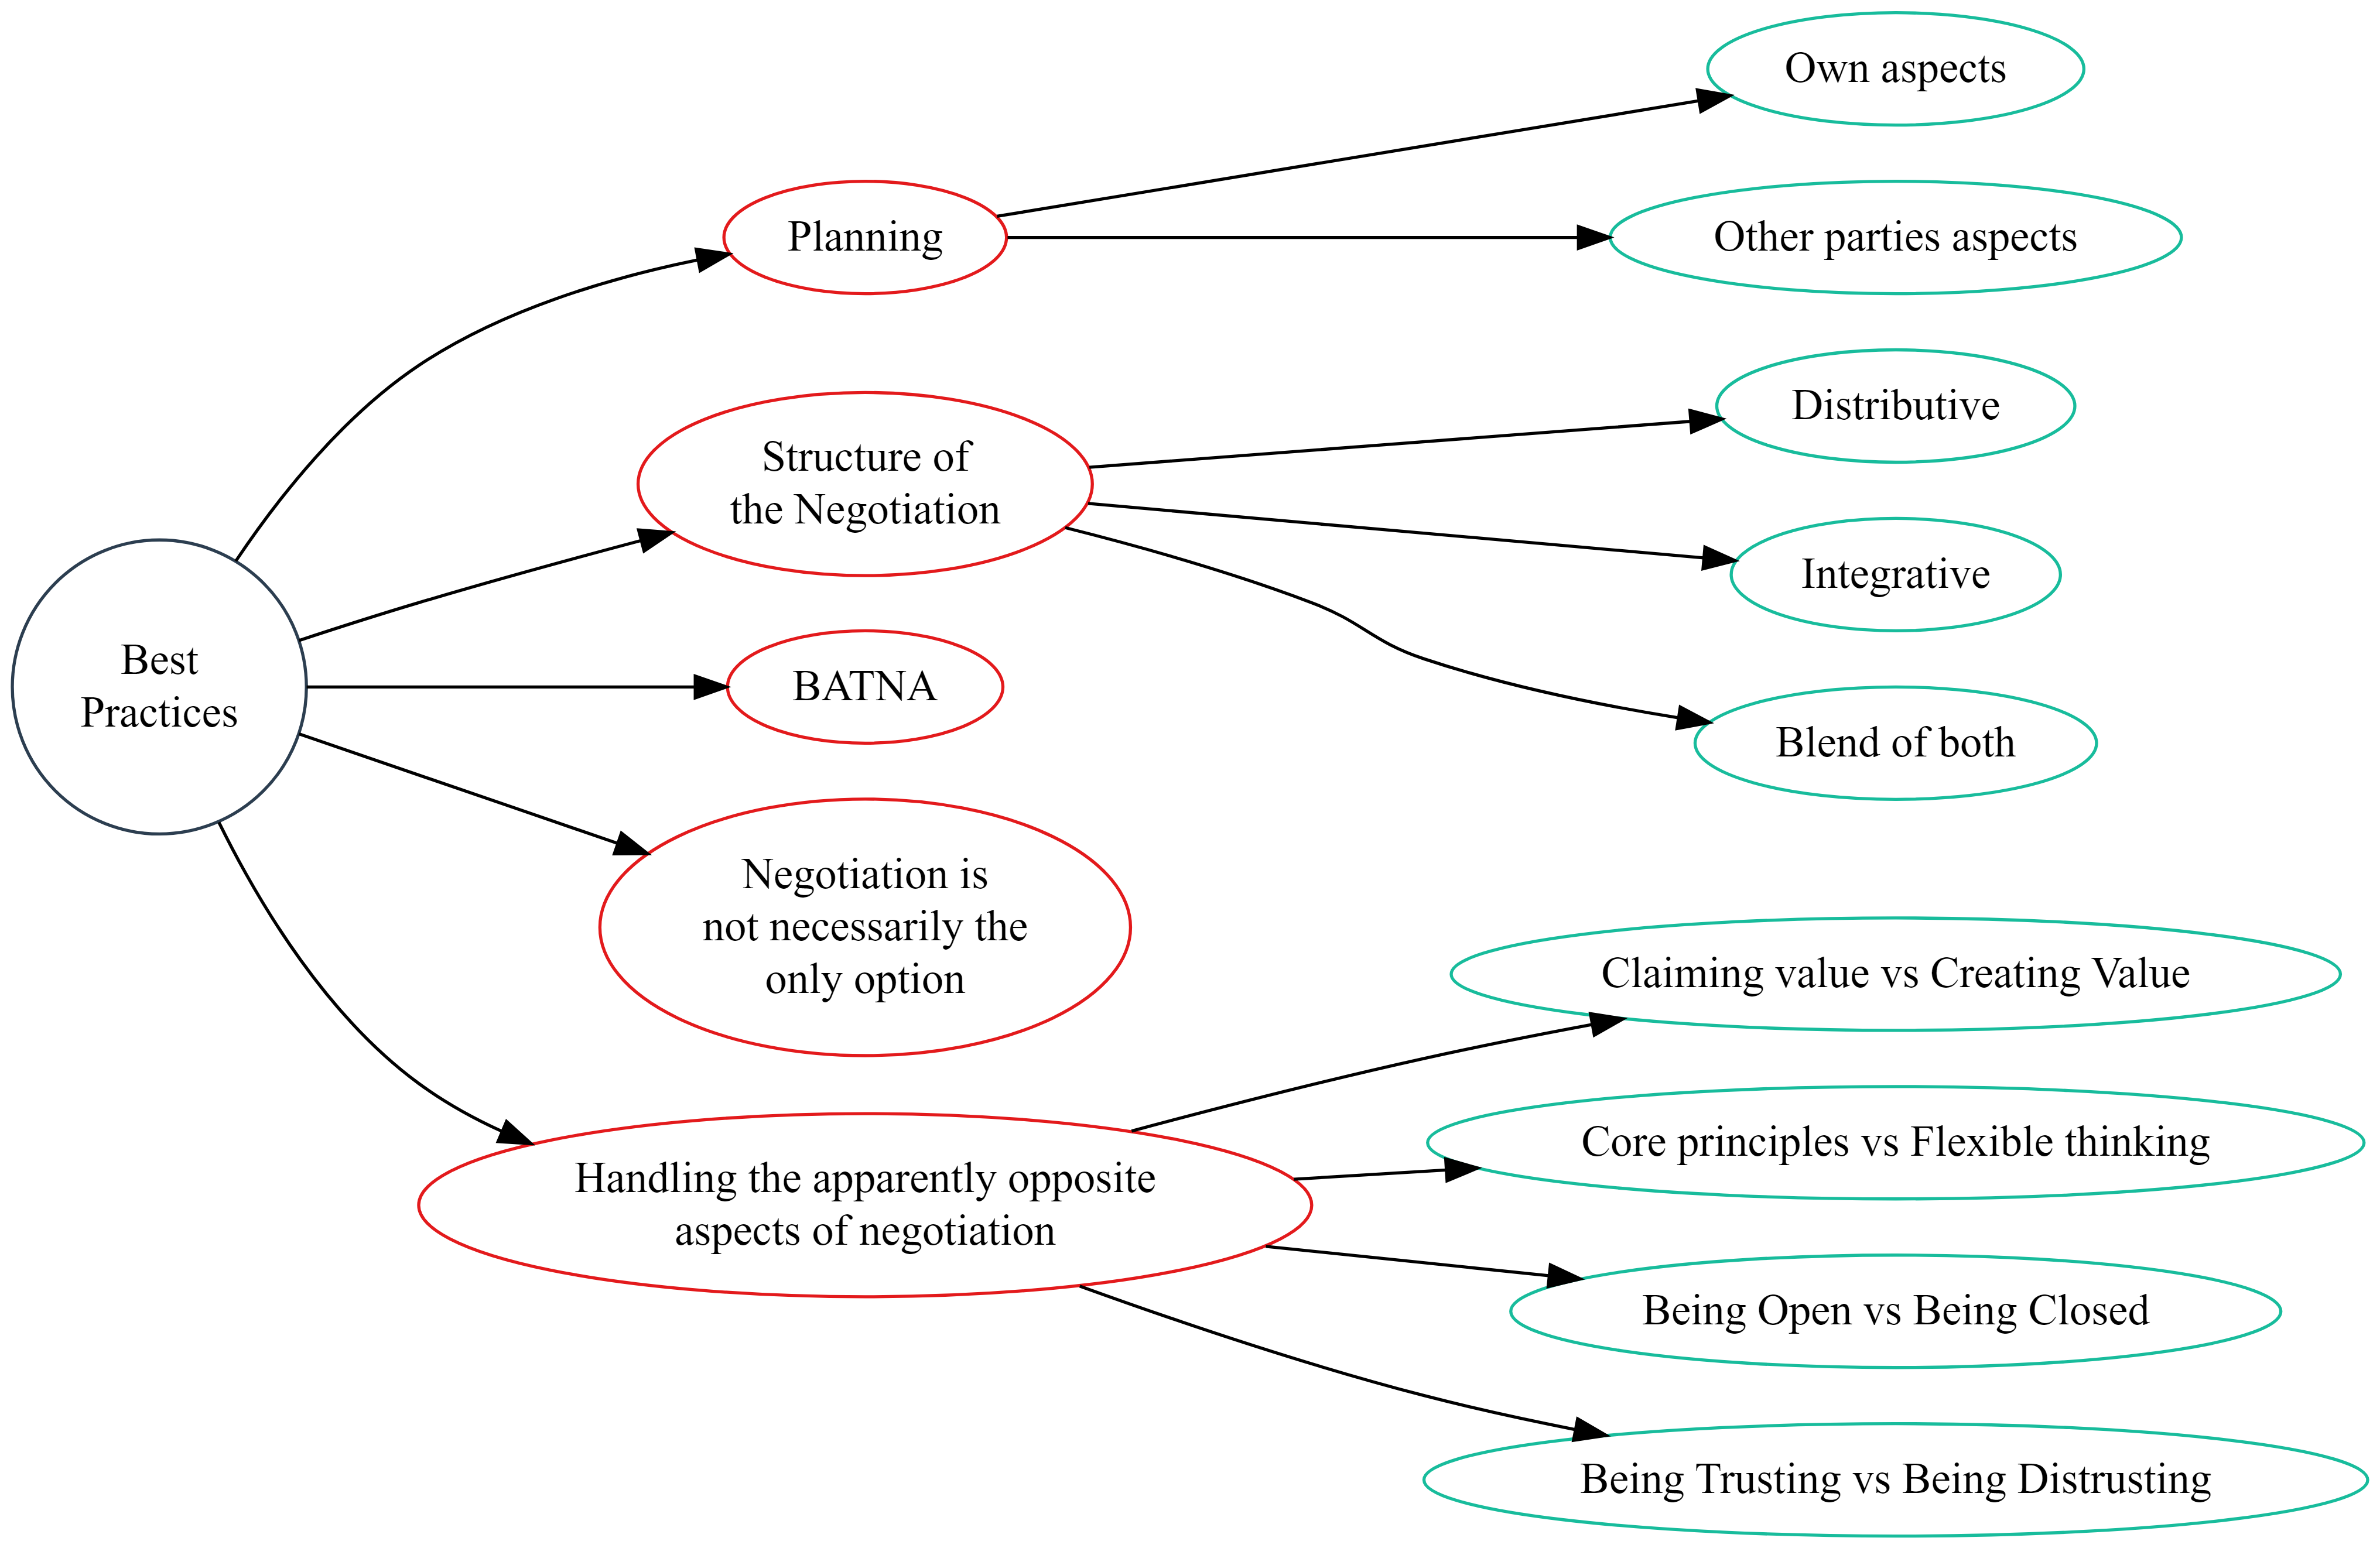
\includegraphics[width=4.5in,height=2.5in]{009_best_practices_files/figure-beamer/dot-figure-1.png}

}

\caption{\label{fig-best-practices-for-negotiators-1}Best Practices for
Negotiators (\citeproc{ref-lewicki_negociacion_2024}{Lewicki, Barry, and
Saunders 2024}, pp 557-565)}

\end{figure}%
\end{frame}

\begin{frame}{}
\phantomsection\label{section-12}
\begin{figure}

\centering{

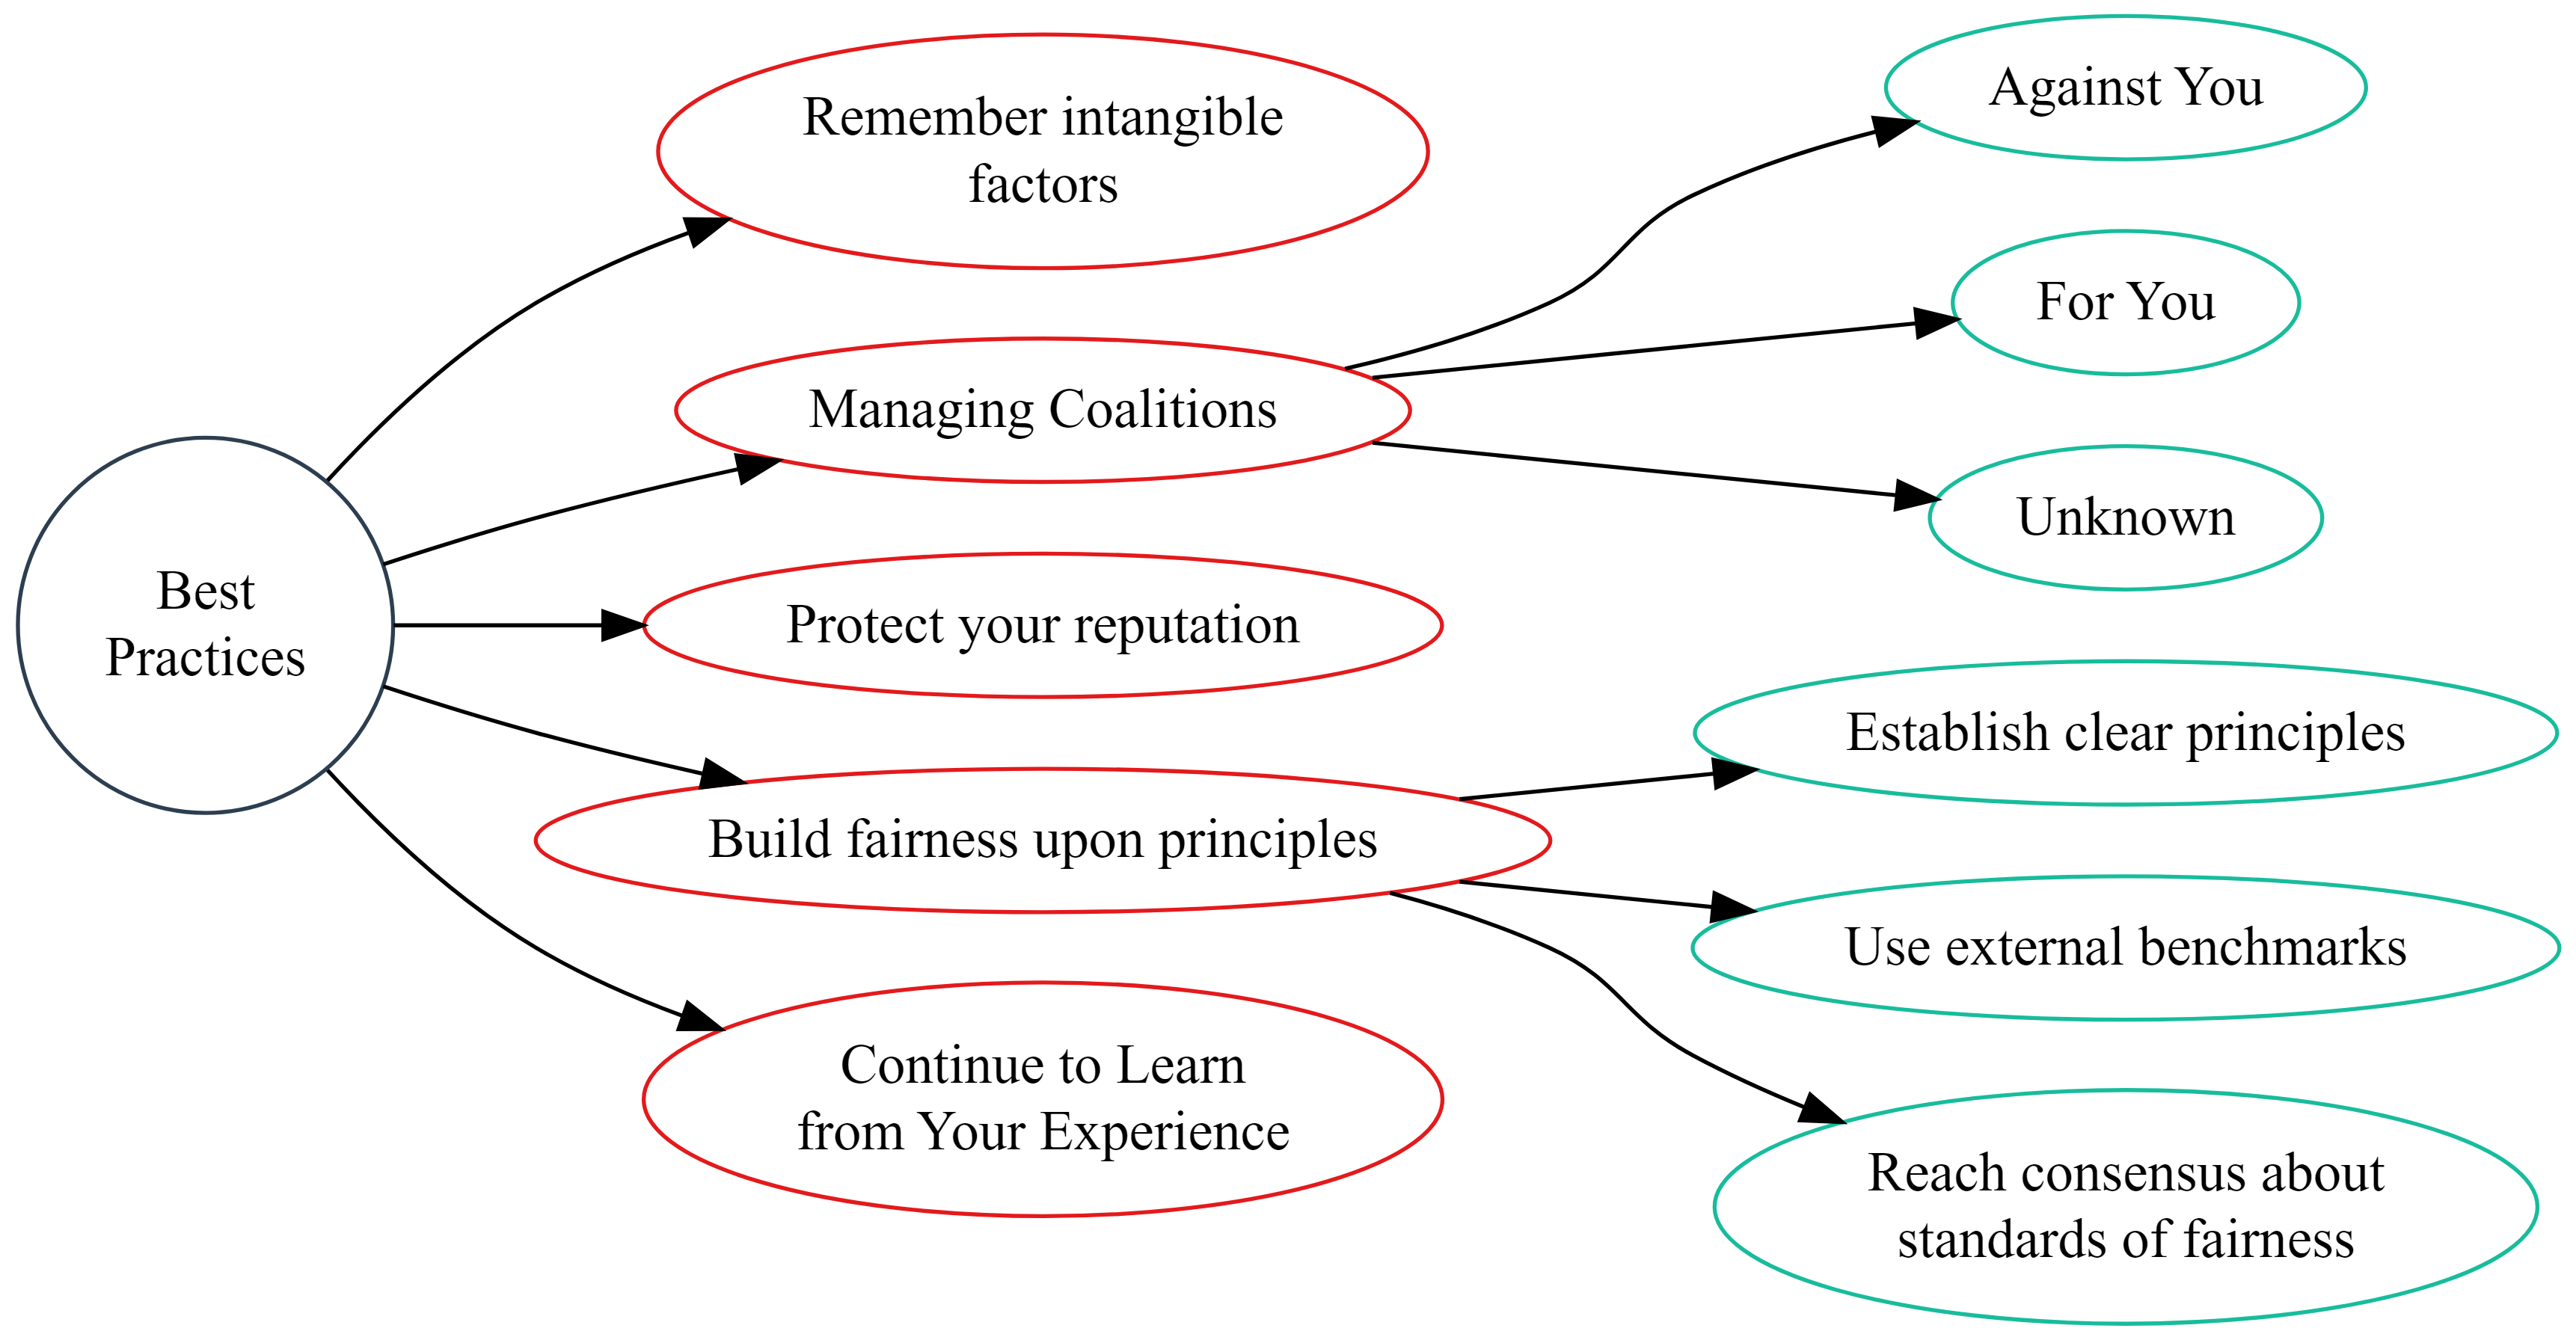
\includegraphics[width=4.5in,height=2.5in]{009_best_practices_files/figure-beamer/dot-figure-2.png}

}

\caption{\label{fig-best-practices-for-negotiators-2}Best Practices for
Negotiators (\citeproc{ref-lewicki_negociacion_2024}{Lewicki, Barry, and
Saunders 2024}, pp 557-565)}

\end{figure}%
\end{frame}

\section{What next?}\label{what-next}

\begin{frame}{}
\phantomsection\label{section-13}
\begin{itemize}
\item
  Book

  \begin{itemize}
  \tightlist
  \item
    Raiffa, H., \& Richardson, J. (2007). Negotiation analysis: The
    science and art of collaborative decision making. Cambridge (Mass.:
    Harvard University Press.
  \end{itemize}
\item
  Online resource

  \begin{itemize}
  \tightlist
  \item
    The Program on Negotiation (PON): \url{https://www.pon.harvard.edu/}
  \end{itemize}
\end{itemize}
\end{frame}

\begin{frame}{}
\phantomsection\label{section-14}
\begin{itemize}
\item
  Postgraduate education:

  \begin{itemize}
  \item
    \textbf{UMNG}:
    \url{https://www.umng.edu.co/programas/posgrados/maestria-en-relaciones-y-negocios-internacionales}

    \begin{itemize}
    \tightlist
    \item
      \textbf{Maestría en Relaciones y Negocios Internacionales}:
      Negociación Internacional
    \end{itemize}
  \item
    \textbf{Uniandes}:
    \url{https://administracion.uniandes.edu.co/programas/posgrados/especializacion-negociacion/}

    \begin{itemize}
    \tightlist
    \item
      \textbf{Especialización en Negociación}: programa de la Facultad
      de Administración
    \end{itemize}
  \end{itemize}
\end{itemize}
\end{frame}

\section{Acknowledgments}\label{acknowledgments}

\begin{frame}{}
\phantomsection\label{section-15}
\begin{itemize}
\item
  To my family that supports me
\item
  To the taxpayers of Colombia and the
  \href{https://www.umng.edu.co/estudiante}{\textbf{UMNG students}} who
  pay my salary
\item
  To the \href{https://www.business-science.io/}{\textbf{Business
  Science}} and \href{https://www.rfordatasci.com/}{\textbf{R4DS Online
  Learning}} communities where I learn
  \href{https://www.r-project.org/about.html}{\textbf{R}}
\item
  To the \href{https://www.r-project.org/contributors.html}{\textbf{R
  Core Team}}, the creators of
  \href{https://rstudio.com/products/rstudio/}{\textbf{RStudio IDE}},
  \href{https://quarto.org/}{\textbf{Quarto}} and the authors and
  maintainers of the packages
  \href{https://CRAN.R-project.org/package=tidyverse}{\textbf{tidyverse}},
  \href{https://CRAN.R-project.org/package=knitr}{\textbf{knitr}},
  \href{https://CRAN.R-project.org/package=kableExtra}{\textbf{kableExtra}},
  \href{https://CRAN.R-project.org/package=tinytex}{\textbf{tinytex}}
  for allowing me to access these tools without paying for a license
\item
  To the \href{https://www.kernel.org/category/about.html}{\textbf{Linux
  kernel community}} for allowing me the possibility to use some
  \href{https://static.lwn.net/Distributions/}{\textbf{Linux
  distributions}} as my main
  \href{https://en.wikipedia.org/wiki/Operating_system}{\textbf{OS}}
  without paying for a license
\end{itemize}
\end{frame}

\section*{References}\label{references}
\addcontentsline{toc}{section}{References}

\begin{frame}{References}
\phantomsection\label{refs}
\begin{CSLReferences}{1}{0}
\bibitem[\citeproctext]{ref-lewicki_negociacion_2024}
Lewicki, Roy J., Bruce Barry, and David M. Saunders. 2024.
\emph{Negociación}. 9th ed. McGraw-Hill Education.
\url{https://www-ebooks7-24-com.ezproxy.umng.edu.co/?il=40562}.

\bibitem[\citeproctext]{ref-program_on_negotiation_negotiation_2014}
Program on Negotiation. 2014a. {``Negotiation {Role}-{Play}:
{Three}-{Party} {Coalition} {Exercise} - {Game} {Theory} \&
{Negotiation} {Analytics}.''}
\url{https://www.youtube.com/watch?v=oaOv_iXOvtY}.

\bibitem[\citeproctext]{ref-program_on_negotiation_negotiation_2014-1}
---------. 2014b. {``Negotiation {Role}-{Play}: {Three}-{Party}
{Coalition} {Exercise} - {Game} {Theory} \& {Negotiation}
{Analytics}.''}
\url{https://www.youtube.com/watch?v=O2d6XuDm-ok&feature=emb_title}.

\end{CSLReferences}
\end{frame}




\end{document}
